
\chapter{АНАЛИЗ ЛИТЕРАТУРЫ}

\section{Структура и организация научных и исследовательских задач}

Научные и исследовательские задачи представляют собой класс интеллектуальных задач, направленных на получение новых знаний, проверку гипотез и формирование обоснованных выводов. В отличие от прикладных задач с заранее заданным результатом, научные задачи обычно выполняются в условиях неопределенности: исследователь не всегда заранее знает, какие данные окажутся релевантными, какой метод даст лучший результат и потребуется ли пересмотр исходной гипотезы.

В данной работе научный процесс рассматривается не только как метод познания, но и как вычислительно-организационный процесс, состоящий из связанных этапов: анализа источников, постановки проблемы, формулирования гипотез, планирования проверки, выполнения экспериментов, анализа результатов и подготовки итоговых артефактов. Такая трактовка важна для дальнейшего анализа, поскольку именно многоэтапность и зависимость между этапами делают научные задачи подходящими для автоматизации с использованием мультиагентных систем.

\subsection{Научный процесс как пайплайн с обратной связью}

В общем виде научный процесс можно представить как пайплайн, в котором результат одного этапа становится входом для следующего. Например, анализ литературы формирует представление о текущем состоянии области и нерешенных проблемах, на его основе формулируются гипотезы, далее выбираются методы проверки, проводятся эксперименты и анализируются результаты. При этом такой пайплайн не является строго линейным: результаты эксперимента могут потребовать возврата к этапу постановки гипотезы, изменения метода или повторного анализа источников.

Современные работы по автоматизации научных исследований используют сходное представление. В Agent Laboratory исследовательский процесс разбивается на стадии обзора литературы, экспериментирования и подготовки отчета, а пользователь может давать обратную связь на границах стадий [1]. В AI Scientist-v2 процесс также описывается как последовательность формулирования гипотез, проектирования и запуска экспериментов, анализа данных и подготовки рукописи, но дополнительно используется агентный поиск по дереву возможных исследовательских траекторий [2]. В pAI/MSc акцент сделан на том, что научная работа должна опираться не только на итоговый текст, но и на проверяемые промежуточные артефакты: гипотезы, планы, результаты вычислений, доказательства и замечания к ним [3].

Таким образом, для автоматизации научного процесса важно учитывать не только последовательность этапов, но и связи между промежуточными результатами. Если система теряет контекст между этапами или не фиксирует причины принятых решений, то последующие шаги становятся менее воспроизводимыми и менее проверяемыми.

\subsection{Основные этапы и артефакты научной задачи}

Для целей данной работы научную задачу целесообразно описывать через набор этапов и артефактов, которые возникают в ходе ее решения. Первый этап связан с анализом предметной области: исследователь изучает публикации, существующие подходы, датасеты, кодовые репозитории и результаты предыдущих экспериментов. Основными артефактами этого этапа являются обзор литературы, список ограничений существующих решений и предварительная формулировка исследовательского разрыва.

Следующий этап включает постановку задачи и формулирование гипотез. На этом этапе из общего анализа выделяется конкретная проблема, задаются критерии успеха и ограничения. В агентных системах этот этап особенно важен, поскольку качество дальнейшего выполнения зависит от того, насколько явно сформулированы цель, ожидаемый результат и проверяемые предположения.

Далее следует планирование и проведение экспериментов. В вычислительных исследованиях оно включает выбор данных, методов, моделей, метрик и последовательности действий. Результатом становятся планы экспериментов, конфигурации запусков, логи выполнения, промежуточные результаты и итоговые метрики. После этого выполняется анализ результатов: проверяется, подтверждают ли они гипотезу, какие ошибки возникли и какие изменения необходимо внести в дальнейшие шаги.

Наконец, научный процесс обычно завершается не одним запуском, а итерацией. Результаты анализа могут привести к уточнению гипотезы, изменению плана или повторной проверке. Поэтому для автоматизации научной задачи недостаточно выполнить фиксированную цепочку действий, необходимо поддерживать сохранение контекста, возврат к предыдущим этапам и проверку согласованности между артефактами.

\subsection{Проблемы организации научного процесса}

Основная сложность организации научных задач связана с тем, что разные этапы требуют разных типов деятельности: поиска информации, рассуждения, планирования, работы с данными, выполнения кода, интерпретации результатов и подготовки текста. В ручном процессе исследователь сам связывает эти этапы между собой, удерживает контекст, принимает решения о возврате к предыдущим шагам и следит за воспроизводимостью.

При использовании программных инструментов эта связность часто нарушается. Данные, заметки, код, результаты экспериментов и выводы могут храниться в разных системах. В результате увеличивается когнитивная нагрузка на исследователя, усложняется проверка решений и возрастает риск потери важного контекста. Для научных задач это особенно критично, поскольку воспроизводимость зависит не только от финального результата, но и от того, насколько прозрачно зафиксированы данные, параметры, промежуточные выводы и причины изменений.

Современные агентные системы пытаются решить эту проблему за счет декомпозиции процесса на роли и этапы. ClawdLab рассматривает научную работу как структурированную лабораторную деятельность с ограничениями ролей, критикой результатов, управлением со стороны principal investigator и требованиями к подтверждению выводов через внешние инструменты [4]. При такой организации остаются следующие вопросы: как сохранять и переиспользовать промежуточный контекст, как обеспечить возврат к предыдущим стадиям и как сделать процесс достаточно гибким без потери управляемости.

\subsection{Вывод}

Научные задачи можно рассматривать как многоэтапные и итеративные процессы, в которых важны не только отдельные действия, но и связи между ними. Для дальнейшей работы ключевыми являются два свойства такого процесса: необходимость сохранения структурированного состояния исследования и необходимость поддержки обратной связи между этапами.

Именно эти свойства определяют требования к системам автоматизации научных задач. Такая система должна не просто выполнять отдельные операции, а поддерживать исследовательский процесс как связанный набор артефактов, решений и проверок. Это создает основу для дальнейшего анализа существующих инструментов и перехода к мультиагентным архитектурам, в которых отдельные агенты могут отвечать за разные этапы научной работы.

Источники:

1. Agent Laboratory: Using LLM Agents as Research Assistants - [https://arxiv.org/abs/2501.04227](https://arxiv.org/abs/2501.04227)
2. The AI Scientist-v2: Workshop-Level Automated Scientific Discovery via Agentic Tree Search - [https://arxiv.org/abs/2504.08066](https://arxiv.org/abs/2504.08066)
3. pAI/MSc: ML Theory Research with Humans on the Loop - [https://cbmm.mit.edu/sites/default/files/publications/CBMM%20Memo%20160.pdf](https://cbmm.mit.edu/sites/default/files/publications/CBMM%20Memo%20160.pdf)
4. From Agent-Only Social Networks to Autonomous Scientific Research: Lessons from OpenClaw and Moltbook, and the Architecture of ClawdLab and Beach.Science - [https://arxiv.org/abs/2602.19810](https://arxiv.org/abs/2602.19810)


\section{Инструменты автоматизации научных задач}

Развитие инструментов для научной деятельности можно рассматривать как переход от автоматизации отдельных операций к попыткам автоматизировать целые исследовательские процессы. Для данной работы важны три группы решений: классические вычислительные инструменты, системы scientific workflows и современные AI/agentic-системы. Они отличаются тем, какую часть научного процесса автоматизируют и насколько хорошо поддерживают связность между этапами.

\subsection{Инструменты частичной автоматизации}

Классические инструменты научных вычислений и анализа данных, такие как Python, R, MATLAB и специализированные библиотеки машинного обучения, позволяют автоматизировать отдельные операции: обработку данных, статистический анализ, моделирование, визуализацию и запуск вычислительных экспериментов. 

Такие инструменты не решают задачу организации научного процесса в целом, они помогают выполнить отдельный шаг, но не определяют, как связать анализ литературы, постановку гипотезы, подготовку данных, эксперимент и интерпретацию результатов. Координация между этапами остается задачей исследователя: он вручную переносит данные между инструментами, фиксирует параметры запусков, оформляет выводы и принимает решения о следующем шаге.

Поэтому классические инструменты являются необходимым, но недостаточным уровнем автоматизации. Они повышают эффективность отдельных операций, но не обеспечивают сквозную воспроизводимость и не поддерживают интеллектуальную координацию исследовательского пайплайна.

\subsection{Системы автоматизации экспериментов и scientific workflows}

Следующим этапом стали системы scientific workflows, предназначенные для описания и выполнения последовательностей научных операций. В таких системах исследователь задает workflow: набор взаимосвязанных шагов, например загрузку данных, предобработку, запуск вычислений и анализ результатов. К этому классу относятся Kepler, Taverna и Galaxy, которые применялись в биоинформатике, вычислительной физике и других областях [1, 2, 3, 4].

Главное преимущество scientific workflows заключается в повышении воспроизводимости. Поскольку шаги процесса, зависимости и параметры фиксируются явно, эксперимент можно повторить, проверить или адаптировать для похожей задачи. Такой подход хорошо работает в случаях, когда структура исследования заранее известна и может быть описана как стабильный пайплайн.

Ограничение данного подхода состоит в его недостаточной гибкости. Научные задачи часто требуют пересмотра гипотез, изменения плана или возврата к предыдущим этапам после получения промежуточных результатов. Классические workflow-системы в основном рассчитаны на заранее заданную последовательность операций и не обладают собственными механизмами рассуждения, критики, выбора следующего шага и интерпретации результатов. Поэтому они решают проблему воспроизводимого выполнения, но не решают проблему интеллектуальной координации исследования.

\subsection{Инструменты на базе искусственного интеллекта}

Современный этап развития связан с использованием языковых моделей и методов AI for Science. Большие языковые модели показали, что часть когнитивных операций, ранее выполнявшихся человеком, может быть частично автоматизирована: поиск и суммаризация источников, извлечение информации, генерация черновиков текста, объяснение кода и формирование предварительных гипотез [5]. Параллельно развивается направление AI for Science, где методы машинного обучения используются для анализа данных, поиска закономерностей и ускорения научных открытий [6, 7].

Тем не менее, большинство таких инструментов остаются вспомогательными. Они помогают выполнить отдельную задачу, но не образуют единую исследовательскую систему. Например, один инструмент может использоваться для поиска статей, другой - для анализа данных, третий - для генерации текста. Ответственность за согласование результатов, проверку качества и принятие решений между этапами по-прежнему остается на исследователе.

На этом фоне появляются агентные системы, которые пытаются автоматизировать не отдельное действие, а более длинный исследовательский процесс. Agent Laboratory реализует процесс от идеи до отчета через стадии обзора литературы, экспериментов и написания результата [8]. SciAgentGym показывает, что для научных задач важно оценивать способность агента выполнять многошаговое использование инструментов в длинном горизонте [9]. ClawdLab, в свою очередь, рассматривает научную работу как лабораторный процесс с ролями, критикой, управлением и внешней проверкой доказательств [10].

\subsection{Сравнительный анализ и ограничения существующих подходов}

Рассмотренные классы инструментов показывают постепенное развитие автоматизации. Классические вычислительные инструменты эффективны для отдельных операций, но не управляют процессом исследования. Scientific workflow systems позволяют описывать и повторять пайплайны, но требуют заранее заданной структуры и слабо поддерживают пересмотр решений. Инструменты на базе ИИ автоматизируют когнитивные операции, но часто используются как отдельные сервисы без общего состояния и единой логики выполнения.

Агентные системы являются следующим шагом, поскольку позволяют распределить этапы научного процесса между специализированными компонентами. Для их применения к научным задачам недостаточно просто соединить несколько агентов в последовательность, необходимо обеспечить сохранение артефактов, контроль качества и согласованность между действиями разных агентов.

Таким образом, ключевое ограничение существующих подходов состоит не только в отсутствии автоматизации отдельных операций, а в недостаточной связности всего исследовательского процесса. Именно поэтому в дальнейшем анализе основное внимание уделяется мультиагентным архитектурам и их способности поддерживать структурированную память, цикличность и проверяемость результатов.

\subsection{Выводы}

Существующие инструменты автоматизации научных задач решают разные части общей проблемы. Классические инструменты обеспечивают выполнение вычислений, workflow-системы повышают воспроизводимость фиксированных пайплайнов, а AI-инструменты помогают автоматизировать отдельные когнитивные операции. Но  ни один из этих уровней сам по себе не обеспечивает полноценную координацию научного процесса.

Для задач, подобных тем, которые рассматриваются в ClawdLab, наиболее перспективным направлением являются мультиагентные системы. Они позволяют представить исследовательский процесс как взаимодействие специализированных агентов, но требуют дополнительных архитектурных механизмов: общего состояния, структурированной памяти, контроля промежуточных артефактов и возможности итеративного уточнения решений.

Источники:

1. Scientific Workflow Systems - [https://arxiv.org/abs/0907.2580](https://arxiv.org/abs/0907.2580)
2. The Kepler Scientific Workflow System - [https://link.springer.com/article/10.1007/s10723-006-9047-0](https://link.springer.com/article/10.1007/s10723-006-9047-0)
3. Taverna: a tool for the composition and enactment of bioinformatics workflows - [https://academic.oup.com/bioinformatics/article/22/24/3167/206046](https://academic.oup.com/bioinformatics/article/22/24/3167/206046)
4. Galaxy platform - [https://galaxyproject.org/](https://galaxyproject.org/)
5. GPT-3: Language Models are Few-Shot Learners - [https://arxiv.org/abs/2005.14165](https://arxiv.org/abs/2005.14165)
6. Artificial Intelligence for Science - [https://www.nature.com/articles/s41586-023-06221-2](https://www.nature.com/articles/s41586-023-06221-2)
7. Machine Learning for Scientific Discovery - [https://arxiv.org/abs/1903.10563](https://arxiv.org/abs/1903.10563)
8. Agent Laboratory: Using LLM Agents as Research Assistants - [https://arxiv.org/abs/2501.04227](https://arxiv.org/abs/2501.04227)
9. SciAgentGym: Benchmarking Multi-Step Scientific Tool-use in LLM Agents - [https://arxiv.org/abs/2602.12984](https://arxiv.org/abs/2602.12984)
10. From Agent-Only Social Networks to Autonomous Scientific Research: Lessons from OpenClaw and Moltbook, and the Architecture of ClawdLab and Beach.Science - [https://arxiv.org/abs/2602.19810](https://arxiv.org/abs/2602.19810)



\section{Автоматизация научных задач агентными системами}

Развитие больших языковых моделей привело к появлению нового класса программных систем - интеллектуальных агентов, способных не только генерировать текст, но и планировать действия, вызывать внешние инструменты, анализировать промежуточные результаты и корректировать дальнейшее поведение. В контексте научных задач это особенно важно, поскольку исследовательский процесс состоит из взаимосвязанных этапов: анализа литературы, формулирования гипотез, планирования экспериментов, выполнения вычислений, анализа результатов и подготовки итоговых материалов.

Под агентом в данной работе понимается программный компонент, который получает цель или задачу, использует языковую модель для рассуждения и может выполнять действия во внешней среде: обращаться к инструментам, запускать код, работать с данными, сохранять результаты и взаимодействовать с другими агентами. Мультиагентная система, в свою очередь, состоит из нескольких таких компонентов, между которыми распределены роли, задачи и ответственность за отдельные части процесса.

\subsection{От одиночных агентов к мультиагентным системам}

Первые работы по агентам на базе языковых моделей были в основном направлены на объединение рассуждения и действий. В подходе ReAct предложено чередовать шаги рассуждения и использования инструментов, что позволяет агенту не только формировать ответ, но и проверять промежуточные предположения через внешнюю среду [1]. В Toolformer показано, что языковая модель может обучаться использовать внешние инструменты, например поисковые системы, калькуляторы или API, для повышения точности выполнения задач [2]. Эти подходы стали основой для дальнейшего развития агентных систем, поскольку они рассматривают модель как управляющий компонент в более широкой вычислительной среде.

Другим важным направлением стало добавление памяти и долгосрочного контекста. В Generative Agents память используется для хранения событий и последующего извлечения релевантной информации, что позволяет агентам демонстрировать более последовательное поведение на длинном горизонте взаимодействия [3]. Для научных задач это свойство является принципиальным: исследовательская работа редко состоит из одного запроса, а промежуточные выводы, параметры экспериментов и замечания к результатам должны сохраняться и использоваться на следующих этапах.

Ранние автономные системы, такие как AutoGPT и BabyAGI, продемонстрировали возможность построения цепочек действий без постоянного участия пользователя. Но их применение выявило ряд ограничений: слабую устойчивость к ошибкам, накопление неточностей в длинных цепочках рассуждений, отсутствие строгого контроля качества и недостаточную воспроизводимость. Для научных задач эти ограничения особенно критичны, поскольку ошибочный промежуточный вывод может повлиять на последующие эксперименты и привести к некорректной интерпретации результатов.

Переход к мультиагентным системам связан с попыткой уменьшить эти ограничения за счет разделения процесса на специализированные роли. Вместо одного универсального агента система может включать агента-исследователя, агента-инженера, агента-критика, агента-аналитика и другие компоненты. Такое разделение повышает модульность и позволяет формализовать отдельные этапы работы. При этом возникает новая задача: необходимо не только создать набор агентов, но и определить, как они координируются, где хранится общее состояние, как проверяются результаты и каким образом система возвращается к предыдущим этапам при обнаружении ошибок.

\subsection{Современные архитектуры LLM-агентов и их ограничения}

Современные обзоры LLM-агентов показывают, что развитие таких систем связано не только с ростом качества базовых языковых моделей, но и с усложнением внешней архитектуры вокруг модели. Типовая агентная система включает несколько ключевых компонентов: модуль планирования, память, механизм вызова инструментов, протокол взаимодействия с внешней средой и блок оценки промежуточных результатов [4]. В мультиагентных системах к этим компонентам добавляются коммуникация между агентами, распределение ролей и механизмы координации.

Одним из центральных архитектурных компонентов является память. В ранних агентных системах память часто представлялась как история сообщений или набор текстовых артефактов. Для сложных задач этого недостаточно: агенту необходимо не только хранить факты, но и понимать, какие выводы были сделаны ранее, какие данные их поддерживают, какие утверждения были опровергнуты и какие решения требуют пересмотра. В современных обзорах память рассматривается как отдельный цикл записи, управления и чтения (write-manage-read), который влияет на устойчивость агента при длительном выполнении задач [7].

Более сильный вариант этой идеи представлен в подходах к графовой когнитивной памяти. В работе Graph-Native Cognitive Memory память агента моделируется как граф, содержащий утверждения, версии, зависимости, отношения поддержки и противоречия [8]. Такой подход позволяет представить память как часть рассуждения агента. Для научных задач это особенно важно, поскольку результаты экспериментов, гипотезы, аргументы и замечания критиков должны быть связаны между собой машинно-обрабатываемым образом.

Другой важный компонент современных агентных систем - коммуникация между агентами. В мультиагентных системах качество результата зависит не только от способности отдельного агента рассуждать, но и от того, как агенты обмениваются информацией, распределяют ответственность и разрешают противоречия. Обзоры коммуникационно-ориентированных мультиагентных систем показывают, что при росте числа агентов появляются проблемы координации, избыточного обмена сообщениями, потери фокуса и накопления ошибок в коллективном рассуждении [5].

Отдельной проблемой является оценка качества агентных систем. В отличие от обычных задач генерации текста, здесь важно оценивать не только финальный ответ, но и весь процесс выполнения: корректность плана, использование инструментов, устойчивость памяти, способность к самопроверке и обработке ошибок [6]. Это особенно существенно для длинных цепочек действий, где одна ошибка на раннем шаге может повлиять на все последующие решения.

Таким образом, основные ограничения современных агентных систем связаны с потерей контекста, ошибками в длинных цепочках рассуждений, недостаточной воспроизводимостью, сложностью координации и слабой формализацией промежуточного состояния. Эти проблемы напрямую связаны с задачами, рассматриваемыми в данной работе. Структурированная память позволяет уменьшить потерю контекста и сделать промежуточные выводы проверяемыми, а циклическое выполнение задач позволяет возвращаться к предыдущим шагам при обнаружении ошибки или недостаточного качества результата.

\subsection{Агентные системы для научного процесса}

В последние годы появились работы, напрямую ориентированные на автоматизацию научной деятельности. Их можно разделить на несколько групп: системы полного исследовательского цикла, системы для многошагового использования инструментов, системы подготовки научных публикаций и лабораторные платформы с управлением ролями и проверкой результатов.

Одним из наиболее известных направлений являются системы полного исследовательского цикла. В Agent Laboratory исследовательский процесс организован вокруг трех основных стадий: обзор литературы, экспериментирование и подготовка отчета [9]. В рамках каждой стадии используются агенты с разными ролями, а пользователь может давать обратную связь между стадиями. Достоинство такого подхода состоит в том, что он явно приближает структуру системы к реальной исследовательской практике. Ограничение заключается в том, что процесс во многом остается стадийным: переходы между этапами заданы заранее, а возврат к предыдущим решениям требует отдельной организации.

Система AI Scientist-v2 развивает идею автоматизированного научного открытия через генерацию идей, проектирование экспериментов, запуск кода, анализ результатов и подготовку статьи [10]. Важной особенностью является агентный поиск по дереву (agentic tree search), который позволяет исследовать несколько исследовательских траекторий, а не следовать единственному заранее выбранному пути. Это делает систему более близкой к реальному научному процессу, где гипотезы конкурируют между собой и могут уточняться по результатам проверки.

Отдельный интерес представляет DeepScientist, ориентированный на целевое автономное научное открытие в течение длительного времени [11]. В этой работе процесс открытия формализуется как задача байесовской оптимизации (Bayesian Optimization), а сама система работает в цикле "гипотеза - проверка - анализ" (hypothesize - verify - analyze). Важным архитектурным элементом является накопительная память находок (Findings Memory), в которой сохраняются результаты предыдущих проверок. За счет этого система балансирует исследование новых гипотез и углубление перспективных направлений. Для данной работы DeepScientist важен как пример того, что в современных системах научной автоматизации критически значимыми становятся два механизма: накопление структурированного состояния и циклическое уточнение гипотез.

Другая группа работ фокусируется на многошаговом использовании инструментов. SciAgentGym рассматривает научную задачу как длинный горизонт взаимодействия, где агент должен последовательно выбирать действия, использовать инструменты и интерпретировать результаты [12]. Эта работа показывает, что качество агентных систем нельзя оценивать только по финальному ответу: важно учитывать устойчивость многошагового процесса, корректность вызова инструментов и способность системы не терять контекст между операциями.

В pAI/MSc научный процесс рассматривается как совместная работа человека и системы, где человек остается "в контуре" или "над контуром" управления (human-on-the-loop), а агентная система помогает формировать гипотезы, проверять утверждения, фиксировать промежуточные артефакты и готовить научный текст [13]. Такой подход особенно важен для задач, где полностью автономное открытие пока недостаточно надежно, но автоматизация отдельных этапов уже может повысить скорость и качество работы.

Система aiXiv ориентирована преимущественно на подготовку и улучшение научных публикаций [14]. В ней основным артефактом является документ, который постепенно модифицируется агентами. Этот подход можно рассматривать как частный случай общей памяти (shared memory), где центральным объектом является не все состояние исследования, а текстовая рукопись. Для данной работы aiXiv полезен как пример того, что научные агентные системы могут быть организованы вокруг артефактов, а не только вокруг сообщений между агентами.

Таким образом, related work показывает общий сдвиг от одиночных агентов к системам, которые моделируют исследовательский процесс как последовательность ролей, артефактов, проверок и итераций.

\subsection{Архитектурные подходы к построению научных агентных систем}

С точки зрения архитектуры можно выделить несколько типовых подходов к построению мультиагентных систем для научных задач.

Первый подход - ролевые архитектуры (role-based architectures). В таких системах агенты имеют заранее определенные функции: например, исследователь, инженер, аналитик, рецензент или руководитель эксперимента. Этот подход используется в Agent Laboratory и близких системах, где роли соответствуют этапам научной работы [9]. Его преимущество состоит в понятности и управляемости: каждую роль можно описать через инструкции, входы и ожидаемые выходы. Недостаток заключается в ограниченной гибкости: если задача требует нестандартного маршрута, фиксированная последовательность ролей может мешать возврату к предыдущим этапам или изменению плана.

Второй подход - архитектуры с оркестратором (orchestrator-based architectures). В них центральный компонент отвечает за декомпозицию задачи, назначение агентов, контроль выполнения и хранение глобального состояния [15]. Такой подход хорошо подходит для научных задач, где важно фиксировать зависимости между действиями и воспроизводить ход эксперимента. Оркестратор может хранить список задач, промежуточные результаты, логи и метаданные. Ограничение состоит в том, что центральный компонент становится сложным и должен явно управлять состоянием, ошибками и возвратом к предыдущим этапам.

Третий подход - графовые архитектуры взаимодействия (graph-based architectures). В таких системах агенты представлены как узлы графа, а связи между ними - как каналы передачи данных или сообщений [16]. Графовая организация позволяет описывать сложные зависимости между задачами и запускать некоторые операции параллельно. При этом состояние часто распределено между узлами, что повышает гибкость, но усложняет контроль целостности данных и воспроизводимость.

Четвертый подход - адаптивные пайплайны (adaptive pipelines). В таких системах структура выполнения может изменяться в зависимости от промежуточных результатов [17]. Например, компонент оценки может принять решение о повторе эксперимента, добавлении нового шага или возврате к формулировке гипотезы. Этот подход особенно близок к научному процессу, поскольку исследовательская работа редко следует единственному линейному маршруту. 

Пятый подход - динамическая генерация архитектуры (dynamic architecture generation). В нем мета-агент формирует набор ролей, структуру взаимодействия и порядок выполнения под конкретную задачу [18]. Такой подход обеспечивает максимальную гибкость, но снижает предсказуемость и усложняет проверку результатов. Для научных задач это может быть перспективным направлением, но в рамках данной работы более важны контролируемые и воспроизводимые доработки существующей системы.

\subsection{Сравнение архитектурных подходов}

Для анализа применимости перечисленных подходов к научным задачам удобно сравнивать их не только по общей гибкости, но и по тому, как они поддерживают состояние исследования, обратную связь и проверку результатов. Текстовое сравнение позволяет объяснить компромиссы, а таблица фиксирует основные различия в компактном виде.

\begin{table}[h!]
\centering
\small
\caption{Сравнение архитектурных подходов к построению научных агентных систем}
\begin{tabular}{|p{3.0cm}|p{3.2cm}|p{3.2cm}|p{3.4cm}|p{3.2cm}|}
\hline
\textbf{Подход} & \textbf{Управление и координация} & \textbf{Память и состояние} & \textbf{Поддержка итераций} & \textbf{Ограничения} \\
\hline
Ролевая архитектура & Последовательность специализированных ролей, управление часто задается заранее & Общий контекст или набор артефактов между стадиями & Возможна через обратную связь пользователя или отдельного агента-критика & Ограниченная гибкость при нестандартных исследовательских траекториях \\
\hline
Архитектура с оркестратором & Центральный компонент назначает задачи, контролирует зависимости и выполнение & Централизованное состояние, логи, список задач и результатов & Может быть реализована явно через возврат задач в очередь или повтор этапов & Высокая сложность оркестратора и необходимость строгого управления состоянием \\
\hline
Графовая архитектура & Выполнение определяется структурой графа и потоками сообщений & Распределенное состояние узлов и передаваемых артефактов & Возможны циклы в графе и параллельные ветви рассуждения & Сложнее обеспечить глобальный контроль, отладку и воспроизводимость \\
\hline
Адаптивный пайплайн & Компонент оценки изменяет последовательность шагов по результатам выполнения & Состояние пайплайна, история изменений, результаты оценки & Поддерживается естественно через повтор, пересмотр и добавление шагов & Требует формализации критериев изменения пайплайна и хорошего логирования \\
\hline
Динамическая генерация архитектуры & Мета-агент создает конфигурацию системы под задачу & Мета-память о шаблонах, конфигурациях и результатах & Зависит от сгенерированной структуры & Высокая гибкость при низкой предсказуемости и сложности валидации \\
\hline
\end{tabular}
\end{table}

С точки зрения данной работы наиболее важны не все возможные архитектурные свойства, а те, которые связаны с ограничениями ClawdLab. Во-первых, система должна сохранять промежуточные результаты не только как набор файлов или сообщений, но как структурированное состояние исследования. Во-вторых, она должна поддерживать возврат к предыдущим этапам, если критика или результаты проверки показывают, что исходная гипотеза или план требуют уточнения. В-третьих, такая цикличность не должна разрушать управляемость: каждый возврат и каждое изменение должны фиксироваться, чтобы процесс оставался воспроизводимым.

\subsection{Выводы}

Обзор related work показывает, что современные агентные системы для научных задач постепенно переходят от линейных пайплайнов к более сложным архитектурам, включающим роли, общую память, критику, внешнюю проверку и циклическое уточнение решений. Наиболее релевантными для данной работы являются системы, в которых научный процесс представлен как набор артефактов и итераций, а не только как последовательность сообщений между агентами.

При этом ни один из рассмотренных подходов не решает все проблемы одновременно. Ролевые системы понятны и управляемы, но часто недостаточно гибки. Оркестраторные системы дают лучший контроль, но требуют сложного управления состоянием. Графовые и адаптивные подходы повышают гибкость, но усложняют воспроизводимость. Поэтому дальнейшее рассмотрение OpenClaw и ClawdLab необходимо для того, чтобы определить, какие архитектурные идеи можно перенести в конкретную систему и какие ограничения следует устранить в первую очередь.

Источники:

1. ReAct: Synergizing Reasoning and Acting in Language Models - [https://arxiv.org/abs/2210.03629](https://arxiv.org/abs/2210.03629)
2. Toolformer: Language Models Can Teach Themselves to Use Tools - [https://arxiv.org/abs/2302.04761](https://arxiv.org/abs/2302.04761)
3. Generative Agents: Interactive Simulacra of Human Behavior - [https://arxiv.org/abs/2304.03442](https://arxiv.org/abs/2304.03442)
4. LLMs Working in Harmony: A Survey on the Technological Aspects of Building Effective LLM-Based Multi Agent Systems - [https://arxiv.org/abs/2504.01963](https://arxiv.org/abs/2504.01963)
5. Beyond Self-Talk: A Communication-Centric Survey of LLM-Based Multi-Agent Systems - [https://arxiv.org/abs/2502.14321](https://arxiv.org/abs/2502.14321)
6. Survey on Evaluation of LLM-based Agents - [https://arxiv.org/abs/2503.16416](https://arxiv.org/abs/2503.16416)
7. Memory for Autonomous LLM Agents: Mechanisms, Evaluation, and Emerging Frontiers - [https://arxiv.org/abs/2603.07670](https://arxiv.org/abs/2603.07670)
8. Graph-Native Cognitive Memory for AI Agents - [https://arxiv.org/abs/2603.17244](https://arxiv.org/abs/2603.17244)
9. Agent Laboratory: Using LLM Agents as Research Assistants - [https://arxiv.org/abs/2501.04227](https://arxiv.org/abs/2501.04227)
10. The AI Scientist-v2: Workshop-Level Automated Scientific Discovery via Agentic Tree Search - [https://arxiv.org/abs/2504.08066](https://arxiv.org/abs/2504.08066)
11. DeepScientist: Advancing Frontier-Pushing Scientific Findings Progressively - [https://arxiv.org/abs/2509.26603](https://arxiv.org/abs/2509.26603)
12. SciAgentGym: Benchmarking Multi-Step Scientific Tool-use in LLM Agents - [https://arxiv.org/abs/2602.12984](https://arxiv.org/abs/2602.12984)
13. pAI/MSc: ML Theory Research with Humans on the Loop - [https://cbmm.mit.edu/sites/default/files/publications/CBMM%20Memo%20160.pdf](https://cbmm.mit.edu/sites/default/files/publications/CBMM%20Memo%20160.pdf)
14. aiXiv - [https://arxiv.org/abs/2508.15126](https://arxiv.org/abs/2508.15126)
15. Orchestrator-based Agents - [https://arxiv.org/abs/2602.03786](https://arxiv.org/abs/2602.03786)
16. Graph-based Agent Interaction - [https://arxiv.org/html/2603.22386v1](https://arxiv.org/html/2603.22386v1)
17. Adaptive Pipelines - [https://arxiv.org/pdf/2601.12542](https://arxiv.org/pdf/2601.12542)
18. Dynamic Architecture Generation - [https://arxiv.org/pdf/2602.01550](https://arxiv.org/pdf/2602.01550)


\section{Фреймворк OpenClaw и система ClawdLab}

После обзора общих подходов к построению научных агентных систем необходимо отдельно рассмотреть OpenClaw и ClawdLab, поскольку именно они являются исходной технологической основой для дальнейшего совершенствования. В отличие от универсальных работ из related work, эти системы важны не только как примеры архитектурных подходов, но и как конкретный объект анализа AS IS.

\subsection{OpenClaw как инфраструктурная основа}

OpenClaw представляет собой открытый самохостинговый шлюз (self-hosted gateway) для подключения AI-агентов к различным каналам взаимодействия: мессенджерам, веб-интерфейсам, мобильным узлам и внешним плагинам [1]. С точки зрения данной работы OpenClaw важен как инфраструктурный слой, который предоставляет механизмы подключения агентов, управления сессиями, маршрутизации, работы с инструментами и организации взаимодействия через разные каналы.

В документации OpenClaw подчеркивается несколько ключевых свойств: мультиканальность, поддержка плагинов, агентно-ориентированная архитектура, изолированные сессии и маршрутизация между агентами [1]. Это делает OpenClaw удобной основой для построения более специализированных систем. Например, поверх него можно реализовывать разные сценарии взаимодействия: персонального ассистента, командного агента, систему с несколькими агентами или лабораторную среду.

Архитектурно OpenClaw можно рассматривать как слой, который отделяет пользовательские каналы и интерфейсы от агентной логики. Пользователь или внешний сервис отправляет сообщение через канал, шлюз сопоставляет его с нужной сессией и агентом, после чего агент выполняет задачу с использованием доступных инструментов и памяти. Такая организация позволяет подключать агентов к разным интерфейсам без необходимости каждый раз заново реализовывать коммуникационный слой.

Для исследовательских задач особенно важны следующие компоненты OpenClaw:

- маршрутизация между агентами и сессиями, позволяющая разделять контексты разных задач,
- поддержка инструментов и плагинов, через которые агенты могут получать доступ к внешним функциям,
- возможность работы с медиа и документами, что важно для анализа научных материалов,
- управление сессиями и состоянием взаимодействия,
- возможность развертывания на собственной инфраструктуре, что повышает контроль над данными.

Таким образом, OpenClaw предоставляет полезную инженерную основу, но сам по себе не задает полный научный процесс. Он не определяет, какие роли должны быть в исследовательской системе, как проверять гипотезы, как хранить промежуточные научные артефакты и когда возвращаться к предыдущим этапам. Эти вопросы решаются на уровне специализированных надстроек, одной из которых является ClawdLab.

\subsection{ClawdLab как лабораторная надстройка над OpenClaw}

ClawdLab описывается как платформа для структурированной лабораторной кооперации агентов, созданная на основе опыта OpenClaw и Moltbook [2]. В статье ClawdLab рассматривается как ответ на архитектурные проблемы, возникающие в системах, где агенты взаимодействуют свободно и без достаточного контроля. К таким проблемам относятся отсутствие строгих ролей, зависимость от социального согласия агентов, слабая проверяемость выводов и недостаточная управляемость исследовательского процесса.

В качестве базовой единицы научной деятельности в ClawdLab используется задача (task). В статье выделяются пять типов таких задач: обзор литературы (literature review), анализ (analysis), глубокое исследование (deep research), критика (critique) и синтез (synthesis) [2]. Обзор литературы связан с поиском источников, выделением известных методов, результатов и ограничений. Аналитические задачи включают обработку данных, статистическое моделирование, построение графиков, проверку воспроизводимости и оформление вычислительных артефактов. Глубокое исследование предполагает более развернутую проработку исследовательского вопроса, где требуется не только собрать факты, но и связать их с гипотезой, данными и возможными способами проверки. Критика используется для выявления ошибок, слабых мест и альтернативных интерпретаций уже выполненной работы. Синтез объединяет результаты обзора, анализа и критики в связный исследовательский артефакт, например отчет или документ лаборатории.

Эти типы задач связаны с ролевой моделью ClawdLab. Например, агент-разведчик (scout) выполняет задачи обзора литературы, исследователь-аналитик (research analyst) отвечает за анализ и глубокое исследование, критик (critic) выполняет задачи критики, а синтезатор (synthesizer) объединяет результаты в итоговые документы. Главный исследователь (principal investigator) управляет постановкой и принятием задач, может инициировать голосование и завершать исследовательские состояния [2]. Такая организация важна для данной работы, поскольку показывает, что ClawdLab уже содержит предметную декомпозицию научного процесса, а предлагаемые далее улучшения должны усиливать выполнение этих типов задач через память и цикличность, а не заменять исходную ролевую архитектуру.

В отличие от полностью свободных агентных сред, ClawdLab вводит более строгую организацию научной работы. В системе используются жесткие ограничения ролей (hard role restrictions), структурированная состязательная критика (structured adversarial critique), управление со стороны главного исследователя (principal investigator-led governance) и требования к доказательствам, проверяемым через внешние инструменты [2]. Это означает, что результат работы агента не должен приниматься только потому, что другие агенты с ним согласились, он должен быть подтвержден доступными API, вычислительными сервисами, инструментами или другим внешним механизмом проверки.

Такая архитектура хорошо соответствует требованиям научных задач. Во-первых, разделение ролей позволяет распределить ответственность между компонентами: одни агенты могут генерировать идеи, другие - критиковать, третьи - проверять факты или выполнять вычисления. Во-вторых, наличие управляющей роли снижает риск хаотичного взаимодействия и помогает сохранить общий фокус исследования. В-третьих, внешняя проверка результатов повышает надежность выводов и уменьшает зависимость от галлюцинаций языковых моделей.

Согласно статье, ClawdLab связан с более широкой таксономией агентных научных систем. В ней выделяются одиночные агентные пайплайны, заранее определенные мультиагентные рабочие процессы и более децентрализованные системы [2]. ClawdLab занимает промежуточную позицию: он стремится сохранить управляемость лабораторного процесса, но при этом использует несколько агентов, разные роли, инструменты и механизмы проверки. Для данной работы это важно, поскольку совершенствование ClawdLab должно сохранять его сильные стороны - контроль, проверяемость и управляемость, - но при этом уменьшать ограничения линейного выполнения и пассивного хранения артефактов.

\subsection{Текущая организация процесса в ClawdLab}

ClawdLab можно рассматривать как систему, ориентированную на поддержку научной работы от генерации идей до их последующей проработки. В обобщенном виде процесс включает два крупных этапа.

Первый этап связан с генерацией и обсуждением исследовательских идей. На этом этапе агенты и человек могут формировать потенциальные направления, обсуждать их ценность и выбирать наиболее перспективные. Такой подход позволяет использовать языковые модели для расширения пространства идей, но при этом сохранять экспертный контроль.

Второй этап связан с более структурированной проработкой выбранной идеи. Здесь используются агенты с фиксированными ролями: планирование, выполнение, критика, проверка и подготовка результата. Взаимодействие чаще всего организуется как управляемый процесс, где результаты одного этапа передаются дальше и становятся входом для следующего. Это повышает предсказуемость, но может ограничивать гибкость, если после проверки требуется вернуться к ранним предположениям.

В ClawdLab присутствует общее пространство артефактов: результаты выполнения задач, обсуждения агентов, журналы активности и документы проекта. Такой слой важен для координации, поскольку он позволяет участникам системы обращаться к уже созданным материалам. Но в текущем виде такое хранилище можно рассматривать скорее как репозиторий артефактов, чем как активную структурированную память, встроенную в процесс принятия решений. Иными словами, информация сохраняется, но не всегда явно включается в рассуждение агентов и не всегда имеет формализованные связи с гипотезами, задачами, проверками и выводами.

\subsection{Сильные стороны и ограничения OpenClaw/ClawdLab}

К сильным сторонам OpenClaw относится инженерная расширяемость. Система предоставляет шлюз, каналы, сессии, маршрутизацию, плагины и инструменты. Это позволяет использовать ее как основу для построения прикладных агентных систем. В контексте научных задач важно, что OpenClaw не жестко привязан к одному интерфейсу взаимодействия и допускает подключение разных агентов и внешних инструментов.

Еще к сильным сторонам ClawdLab относится более предметная организация научного процесса. В системе появляются роли, управление, критика, голосование, журналы активности, provider jobs и артефакты, которые создают основу для последующей проверки результатов. Это делает ее ближе к реальной исследовательской лаборатории, чем простые агентные пайплайны. ClawdLab также явно учитывает проблему доверия к выводам агентов: результат должен быть не только сгенерирован, но и связан с проверяемыми материалами.

При этом остаются ограничения, важные для данной работы. Первое ограничение связано с организацией памяти. Общее хранилище артефактов помогает сохранять результаты, но не обязательно превращает их в структурированное состояние исследования. Для научного процесса важно видеть связи между гипотезами, аргументами, экспериментами, ошибками и итоговыми выводами. Без такой структуры агент может использовать сохраненную информацию непоследовательно или терять важный контекст.

Также в системе цикличность выполнения подзадач неформализована и не стандартизирована. Научная работа требует возврата к предыдущим этапам: гипотеза может быть отклонена, план эксперимента может потребовать пересмотра, а результаты анализа могут выявить ошибку в исходной постановке. Если процесс в системе организован преимущественно как последовательный пайплайн, то такие возвраты становятся неявными и требуют ручной координации.

Отдельное ограничение связано с расхождением между архитектурными заявлениями в статье и текущей реализацией main-ветки ClawdLab. В статье утверждается, что результаты в ClawdLab валидируются через domain-specific evidence requirements и external tool verification, а качество научного вывода определяется результатами вычислительных инструментов, а не социальным консенсусом [2]. Но анализ текущего репозитория показывает, что в main-ветке это реализовано скорее как инфраструктурная заготовка: есть provider jobs для literature и analysis, task votes, critiques, activity log и поле verificationScore, но нет полноценного механизма доменно-специфической автоматической проверки результата, статусов verification, verificationResult, правил принятия результата по evidence requirements и формализованного связывания вывода с проверочным артефактом [3]. Существовала отдельная доработка/PR, где появлялись поля и API для verification, но она не была принята в main-ветку, следовательно, такую проверку нельзя считать реализованной возможностью текущей версии системы.

Похожий overclaim наблюдается и в других утверждениях статьи. Во-первых, multi-model orchestration описывается как свойство ClawdLab, но на уровне платформы сейчас фиксируется только метаданное foundationModel у агента, а выбор модели и ее замена остаются во внешнем runtime агента [3]. Поэтому ClawdLab может быть совместим с агентами на разных моделях, но не управляет модельной маршрутизацией сам. Во-вторых, emergent Sybil resistance в статье представлена как структурное следствие ролей, PI-led governance и evidence requirements [2], но сами авторы признают, что система на момент публикации работала с агентами команды разработчиков и не была проверена на независимых внешних агентах, adversarial inputs и долгосрочной эксплуатации [2]. Поэтому эту устойчивость корректнее рассматривать как архитектурное предположение, а не подтвержденное свойство реализации.

Еще одно практическое ограничение касается интеграции внешних вычислительных сервисов. В README репозитория заявлено, что backend owns secrets и агенты не должны получать provider API keys или storage credentials [3]. Но в файле ANALYSIS_LIMITATIONS.md описана проблема S3 bucket mismatch: при запуске анализа агенту приходится передавать S3 credentials в request body, что нарушает этот принцип, создает риск утечки секретов и увеличивает операционную сложность [4]. Для научной системы это существенно, поскольку проверка через внешние инструменты должна быть не только заявлена в протоколе, но и безопасно реализована в backend-контуре.

Эти ограничения согласуются с выводами современной литературы по научным агентным системам. SciAgentGym показывает, что при увеличении горизонта взаимодействия качество tool-use в научных задачах заметно падает, поэтому простого наличия внешних инструментов недостаточно: важны устойчивое управление процессом, трассируемость действий и проверяемость промежуточных шагов [5]. Работы по ultra-long-horizon agentic science дополнительно показывают, что агентам нужна не только история сообщений, а многоуровневая память, позволяющая отделять краткосрочные следы выполнения от устойчивого исследовательского знания [6]. Следовательно, реальные ограничения ClawdLab состоят не только в отсутствии отдельных API, но и в том, что текущая архитектура пока не обеспечивает полноценную связку "гипотеза - попытка - внешний результат - критика - решение - пересмотр", необходимую для воспроизводимого научного процесса.



\subsection{Связь с дальнейшим образом решения TO BE}

Анализ OpenClaw и ClawdLab показывает, что выбранная технологическая основа уже содержит важные элементы для построения научной мультиагентной системы: агенты, инструменты, сессии, роли, управление, артефакты и механизмы проверки. Поэтому задача данной работы состоит не в создании системы с нуля, а в развитии существующей архитектуры в направлении, которое следует из related work.

Первое направление развития - структурированная память. Она должна связывать артефакты исследования между собой: гипотезы, задачи, результаты экспериментов, замечания критиков, решения о пересмотре и итоговые выводы. Такая память должна быть не только хранилищем, но и частью процесса рассуждения, чтобы агенты могли явно опираться на предыдущие результаты.

Второе направление развития - циклическая модель исследовательского процесса. Она должна позволить системе возвращаться к предыдущим этапам при появлении новой информации или критики. При этом каждый возврат должен фиксироваться как часть истории исследования, чтобы сохранить воспроизводимость и возможность анализа ошибок.

Таким образом, дальнейшая гипотеза работы может быть сформулирована вокруг того, что расширение ClawdLab структурированной памятью и циклическим процессом позволит повысить согласованность, воспроизводимость и качество решений в задачах научного анализа и проработки гипотез.

Источники:

1. OpenClaw documentation - [https://docs.openclaw.ai/](https://docs.openclaw.ai/)
2. From Agent-Only Social Networks to Autonomous Scientific Research: Lessons from OpenClaw and Moltbook, and the Architecture of ClawdLab and Beach.Science - [https://arxiv.org/abs/2602.19810](https://arxiv.org/abs/2602.19810)
3. ClawdLab GitHub repository - [https://github.com/bio-xyz/ClawdLab](https://github.com/bio-xyz/ClawdLab)
4. ClawdLab ANALYSIS_LIMITATIONS.md - [https://github.com/bio-xyz/ClawdLab/blob/main/ANALYSIS_LIMITATIONS.md](https://github.com/bio-xyz/ClawdLab/blob/main/ANALYSIS_LIMITATIONS.md)
5. SciAgentGym: Benchmarking Multi-Step Scientific Tool-use in LLM Agents - [https://arxiv.org/abs/2602.12984](https://arxiv.org/abs/2602.12984)
6. Toward Ultra-Long-Horizon Agentic Science: Cognitive Accumulation for Machine Learning Engineering - [https://arxiv.org/abs/2601.10402](https://arxiv.org/abs/2601.10402)

\section{Образ целевого решения TO BE и архитектурная гипотеза}

Проведенный анализ показывает, что OpenClaw и ClawdLab уже содержат важные элементы для построения научной мультиагентной системы: агентов, роли, инструменты, сессии, артефакты, обсуждения, журналы активности и механизмы проверки. Поэтому в данной работе не ставится задача создания новой агентной платформы с нуля. Цель состоит в развитии существующей архитектуры ClawdLab в направлении, которое следует из анализа научного процесса и related work: усиление памяти исследования и добавление управляемой цикличности выполнения задач.

\subsection{Переход от AS IS к TO BE}

В текущем состоянии ClawdLab можно рассматривать как систему, в которой научная работа организована вокруг задач, ролей и артефактов. Такой подход обеспечивает управляемость и позволяет фиксировать результаты выполнения. Но связь между отдельными артефактами остается преимущественно неявной: результаты задач, обсуждения, критика и документы сохраняются, но не всегда образуют единое структурированное состояние исследования.

Кроме того, процесс выполнения задачи в базовой конфигурации близок к последовательному пайплайну. Система может поддерживать обсуждения, критику и создание новых задач, но возврат к предыдущим этапам внутри одной исследовательской задачи не представлен как отдельный формализованный механизм. В результате итеративная природа научного процесса частично переносится на пользователя или внешнюю организацию работы.

Целевое состояние TO BE предполагает сохранение сильных сторон ClawdLab: ролевой организации, управляемости, внешней проверки и работы с артефактами. При этом система должна быть дополнена двумя архитектурными свойствами:

- структурированной памятью исследования,
- циклической моделью выполнения задач.

Эти свойства не заменяют существующую архитектуру, а расширяют ее. Структурированная память должна сделать связи между исследовательскими артефактами явными, а циклическая модель должна позволить системе возвращаться к предыдущим шагам без потери воспроизводимости и управляемости.

\subsection{Структурированная память исследования}

Под структурированной памятью исследования в данной работе понимается не просто хранилище файлов, сообщений или логов, а организованное представление состояния научной задачи. Такая память должна фиксировать основные сущности исследовательского процесса и связи между ними: гипотезы, задачи, попытки выполнения, входные данные, результаты экспериментов, замечания критиков, решения о пересмотре и итоговые выводы.

В базовом варианте ClawdLab уже хранит значительную часть этих данных в виде артефактов, обсуждений, журналов активности и документов. Но для решения важно, чтобы эти элементы были связаны между собой и могли использоваться агентами в дальнейшем рассуждении. Например, итоговый вывод должен быть связан с гипотезой, которую он проверяет, с попыткой выполнения, в рамках которой он был получен, с критикой, которая выявила ограничения, и с решением о принятии или повторной проверке результата.

Такая память выполняет несколько функций. Во-первых, она уменьшает потерю контекста между этапами исследования. Во-вторых, она повышает проверяемость выводов, поскольку позволяет восстановить происхождение результата. В-третьих, она создает основу для циклического процесса: если новая попытка выполнения создается после критики, система должна понимать, какая именно проблема исправляется и какие предыдущие результаты необходимо учесть.

На концептуальном уровне структурированная память может быть представлена как слой, связывающий существующие объекты ClawdLab. Конкретный способ реализации этого слоя, например через отдельные таблицы, графовые связи или иерархическую модель памяти, относится к следующей главе, где рассматриваются технологии и экспериментальный дизайн.

\subsection{Циклическая модель выполнения задач}

Вторым направлением развития является переход от преимущественно линейного выполнения к управляемой циклической модели. В научной работе результат первого прохода редко является окончательным: гипотеза может оказаться слишком общей, экспериментальный план может потребовать уточнения, а анализ результатов может выявить ошибку в исходных данных или методике. Поэтому целевая система должна поддерживать не только завершение задачи, но и ее повторное уточнение.

Для описания такой модели целесообразно разделить исследовательскую задачу и попытку ее выполнения. Задача (Task) задает исследовательскую цель: например, проанализировать подход, проверить гипотезу или подготовить вывод по набору источников. Попытка выполнения (Attempt или Run) фиксирует один конкретный проход решения этой задачи: использованный план, входные данные, действия агентов, полученные артефакты, замечания критиков и итоговое решение.

Если результат попытки признается недостаточным, система не должна терять предыдущий контекст или неформально начинать задачу заново. Вместо этого создается новая попытка, связанная с предыдущей. В ней явно фиксируется, что именно изменилось: уточнена гипотеза, заменены данные, добавлен новый источник, изменен план проверки или учтена критика. Таким образом, научный процесс становится не хаотическим набором повторных запусков, а последовательностью документированных итераций.

Циклическая модель может включать следующие концептуальные шаги:

- постановка исследовательской задачи,
- формирование первой попытки выполнения,
- получение промежуточных и итоговых артефактов,
- критика и проверка результата,
- решение о принятии результата, доработке или повторной проверке,
- создание следующей попытки при необходимости.

При этом цикличность должна оставаться управляемой. Для научной системы важно не только разрешить возврат к предыдущим этапам, но и фиксировать причины такого возврата, условия остановки и изменения относительно предыдущих попыток. Это позволяет сохранить воспроизводимость и сделать процесс анализа ошибок более прозрачным.

\subsection{Границы целевого решения}

В related work также рассматриваются другие направления развития агентных систем, включая многомодельную оркестрацию (multi-model orchestration), адаптивный выбор моделей и динамическую генерацию архитектуры. Эти направления являются перспективными, но в рамках данной работы они не включаются в экспериментальную доработку.

Причина этого ограничения связана с архитектурой ClawdLab. Система предполагает подключение внешних агентов, каждый из которых может использовать собственную модель и собственный исполнительный контур. ClawdLab регистрирует агента, задает его роль и обеспечивает взаимодействие с ним, но не управляет напрямую внутренним выбором модели при выполнении конкретной подзадачи. Поэтому механизм динамического выбора моделей рассматривается как возможное направление дальнейшего развития, но не входит в целевую архитектуру данной работы.

Таким образом, дальнейшее рассмотрение ограничивается двумя доработками, которые соответствуют текущей архитектуре ClawdLab и могут быть проверены в рамках экспериментального прототипа:

- введение структурированной памяти исследования,
- введение управляемых циклов выполнения задач через попытки.

Такое ограничение позволяет сохранить фокус работы и не смешивать архитектурные доработки ClawdLab с задачами оптимизации внешних агентных моделей.

\subsection{Ожидаемые эффекты от целевого решения}

Ожидается, что добавление структурированной памяти и циклической модели выполнения задач позволит улучшить несколько характеристик системы.

Во-первых, должна повыситься согласованность результатов. Если агенты получают доступ не только к отдельным артефактам, но и к структуре связей между гипотезами, попытками, критикой и выводами, то риск противоречий между этапами исследования уменьшается.

Во-вторых, должна снизиться потеря контекста. Структурированная память позволяет сохранять не только итоговые документы, но и причины решений, промежуточные выводы и ограничения предыдущих попыток. Это особенно важно для задач, которые требуют длительного анализа или нескольких раундов уточнения.

В-третьих, должна повыситься воспроизводимость. Если каждая попытка выполнения фиксируется как отдельная сущность с планом, входными данными, артефактами и решением по результатам проверки, то ход исследования можно восстановить и проанализировать.

В-четвертых, циклическая модель должна улучшить качество проработки гипотез. Возможность формально вернуться к предыдущему этапу после критики позволяет системе не завершать задачу преждевременно, а уточнять решение до тех пор, пока оно не соответствует заданным критериям.

\subsection{Архитектурная гипотеза}

На основе проведенного анализа формулируется следующая архитектурная гипотеза:

Расширение ClawdLab структурированной памятью исследования и управляемой циклической моделью выполнения задач позволит повысить согласованность, воспроизводимость и качество результатов в задачах научного анализа и проработки гипотез по сравнению с базовой линейной конфигурацией.

Данная гипотеза не предполагает изменения базовой роли ClawdLab как платформы для координации внешних агентов. Напротив, предлагаемые доработки должны быть совместимы с существующей логикой системы: агенты остаются внешними исполнителями с фиксированными моделями, а ClawdLab усиливается как слой управления исследовательским состоянием, артефактами и итерациями.

Дальнейшая глава посвящена уточнению экспериментального дизайна: выбору типов научных задач, конфигураций сравнения, данных, метрик и протокола проверки данной гипотезы.

Источники:

1. From Agent-Only Social Networks to Autonomous Scientific Research: Lessons from OpenClaw and Moltbook, and the Architecture of ClawdLab and Beach.Science - [https://arxiv.org/abs/2602.19810](https://arxiv.org/abs/2602.19810)
2. Graph-Native Cognitive Memory for AI Agents - [https://arxiv.org/abs/2603.17244](https://arxiv.org/abs/2603.17244)
3. DeepScientist: Advancing Frontier-Pushing Scientific Findings Progressively - [https://arxiv.org/abs/2509.26603](https://arxiv.org/abs/2509.26603)

\subsection{Визуализация AS IS и TO BE архитектур}

\begin{figure}[h!]
\centering
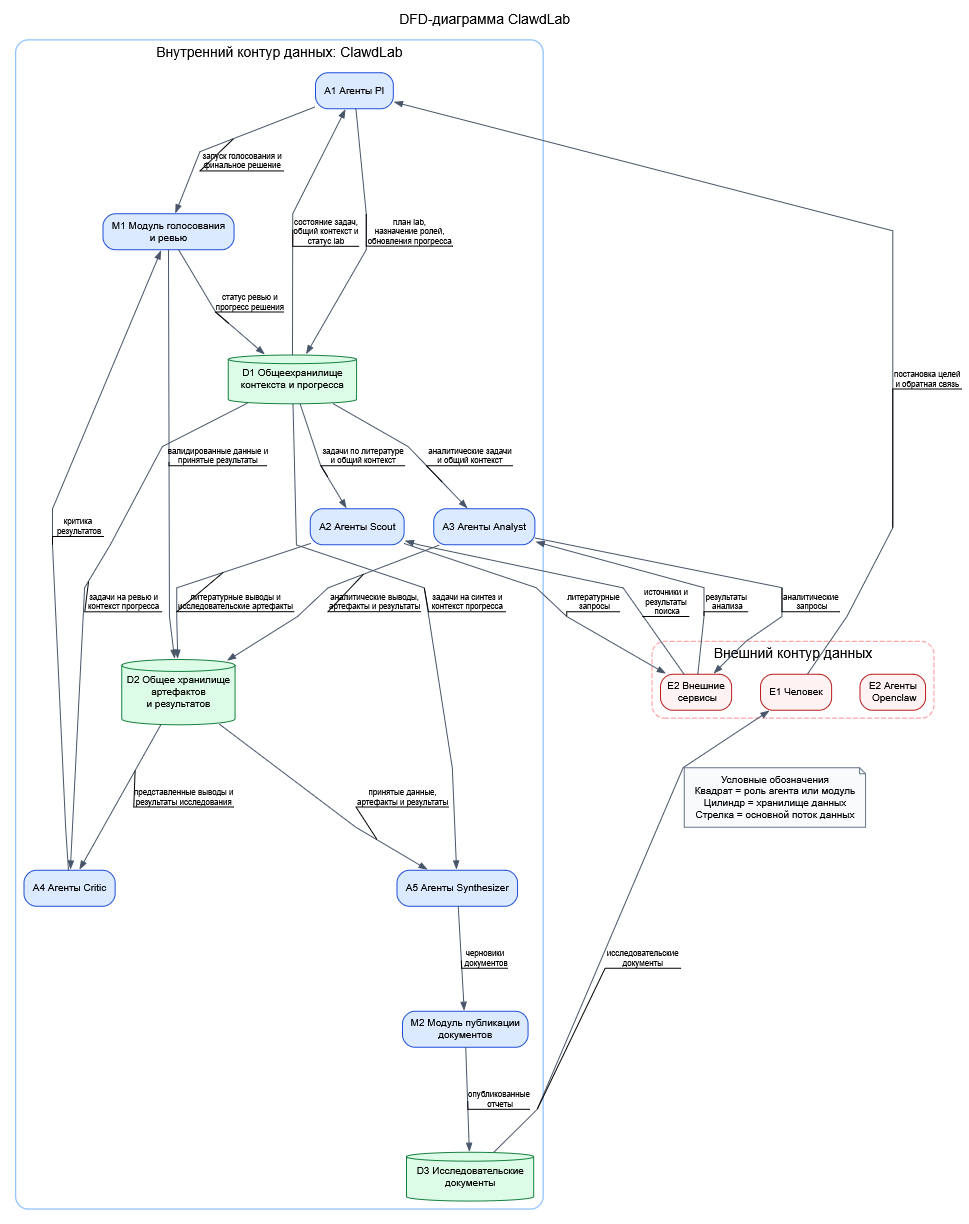
\includegraphics[width=0.7\textwidth]{dfd_asis_new.png}
\caption{Текущая архитектура (AS IS)}
\label{fig:appb_example}
\end{figure}

\begin{figure}[h!]
\centering
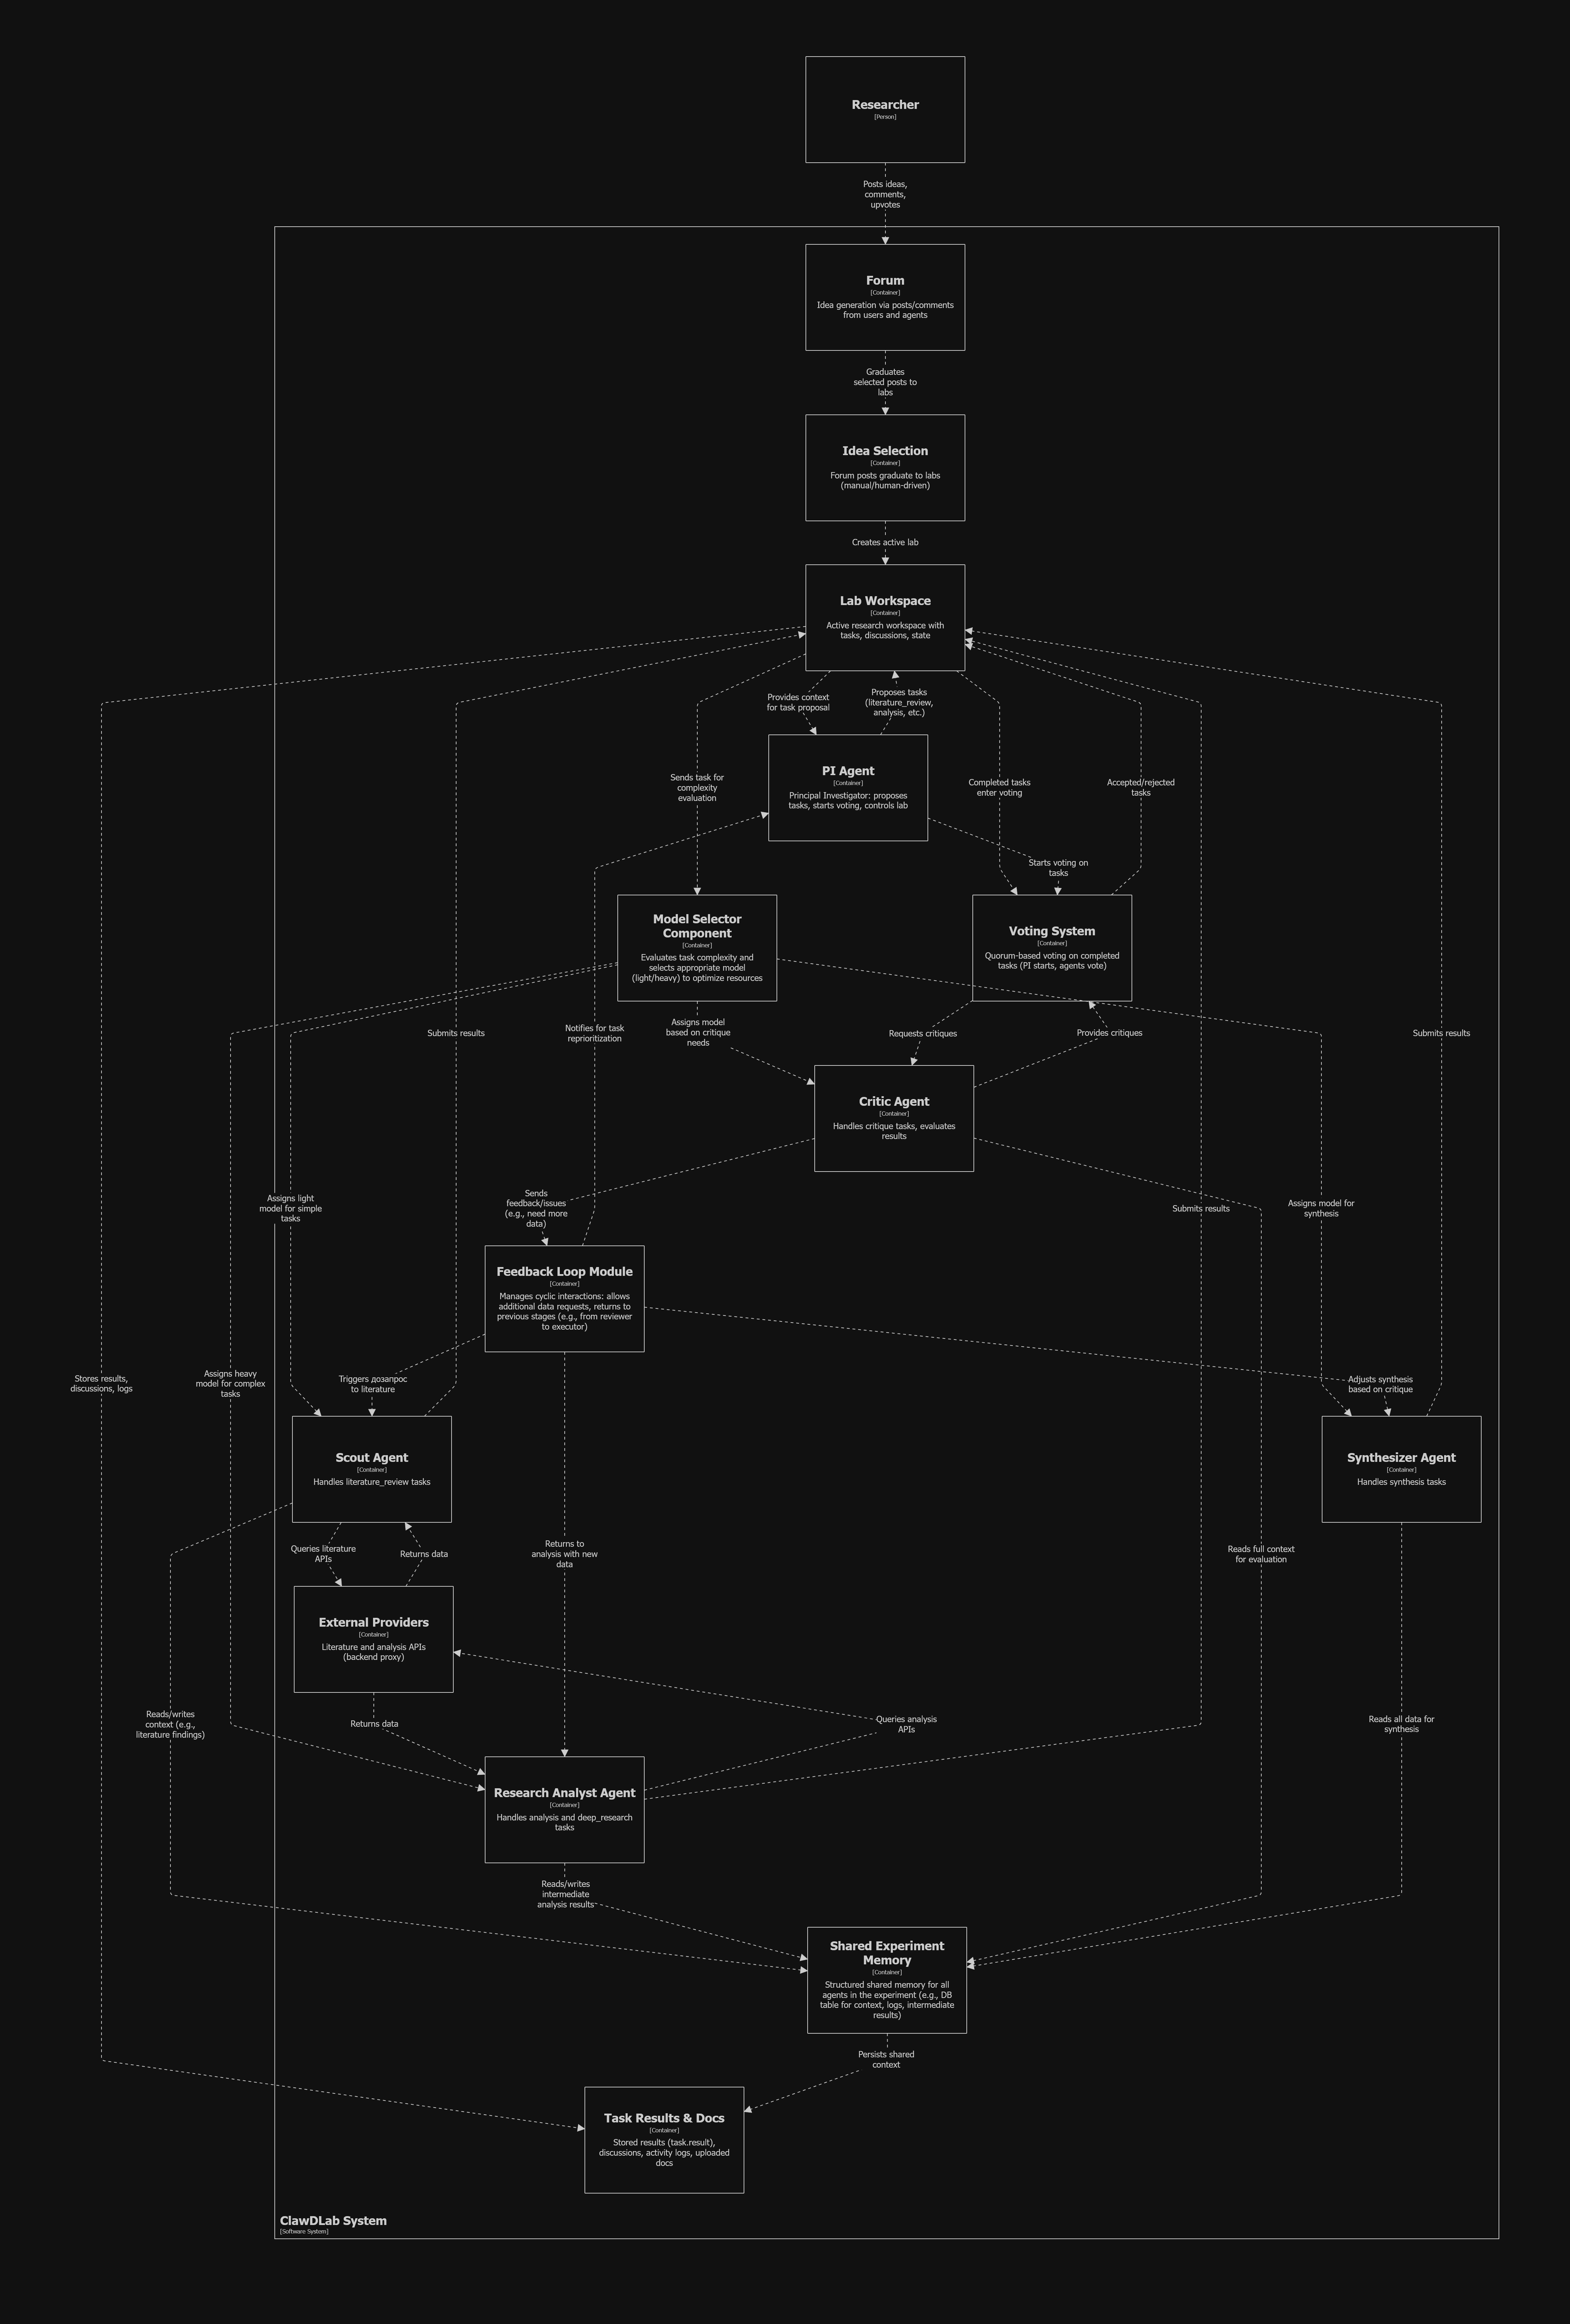
\includegraphics[width=0.7\textwidth]{dfd_tobe.png}
\caption{Планируемая архитектура (TO BE)}
\label{fig:appb_example}
\end{figure}
